\chapter{Introduction}\label{chap:intro}

\section{An example}\label{sec:example}

We start with an example to illustrate the problem central to this thesis.

A number $m$ of containers arrive at a shipping center. It is noted
that all containers are at most $66$ percent full. The items in the
containers are too numerous to be individually labeled, yet all items
must be unpacked and scanned for illicit and dangerous material. After
the scanning, the items arrive at a conveyor belt one by one and they must
be speedily repackaged into the original containers for further shipping.

Our question is: Does there exist a fast computer program which can
repackage the items into the original containers without any
reassignments?

We will settle our central question later in the thesis in the
affirmative (the program exists). Before proceeding with the formal
definitions, let us consider where the difficulty of this problem
lies.

First, let us imagine that we are in the same shipping center, but in
this case we receive two $99$ percent loaded containers. Suppose that
the first item arriving through the scanner is of size $50\%$. We can
choose either container for it, and it is clearly not a wrong choice,
as they are identical.

After storing the first item, a second item arrives through the
scanner, this one of size $47\%$ of the size of the container. We have
a choice to make: do we pack it with the first item or not? See
Figure~\ref{fig:ninetynine} for illustration.

\begin{figure}[th]
\begin{center}
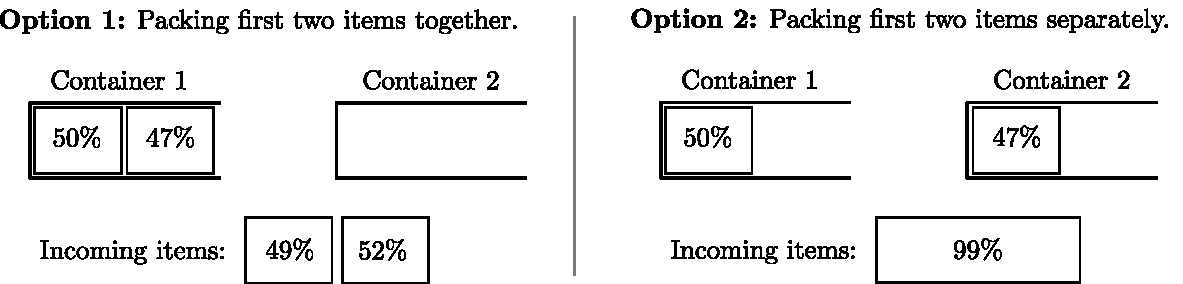
\includegraphics[width=\textwidth]{img/ninetynine.pdf}
\end{center}
\caption{Two possible choices for repacking containers that are $99\%$ full.}
\label{fig:ninetynine}
\end{figure}


A quick thought gives us that there is no good choice here: if we pack
it with the first item, we get a container that is 97 percent loaded,
but then, to our dismay, we receive two items of sizes $49\%$ and
$52\%$, respectively -- and those cannot be packed together. On the
other hand, if we pack the first two items separately into two
containers, we can find that the third item is a large crate taking up
$99\%$ of the container's size, and we have no more containers to
choose from!

\paragraph{A lower bound.} In the last few paragraphs, we have seen
that repacking two containers that are $99\%$ full is impossible
without additional information on their contents. Can we actually get
a lower number than $99\%$ using only simple ideas? The answer is yes:
we can show that we cannot repack two containers that are strictly
more than $75\%$ full. The thought process is explained in Figure~\ref{fig:example-lowerbound}.

The key decision of any algorithm (for containers loaded below $75\%$,
where a repacking algorithm might exist) is then whether to pack
sizable items together and increase the total loaded volume of one
container, or pack them separately to avoid a potentially unsolvable
situation.

\begin{figure}[th]
\begin{center}
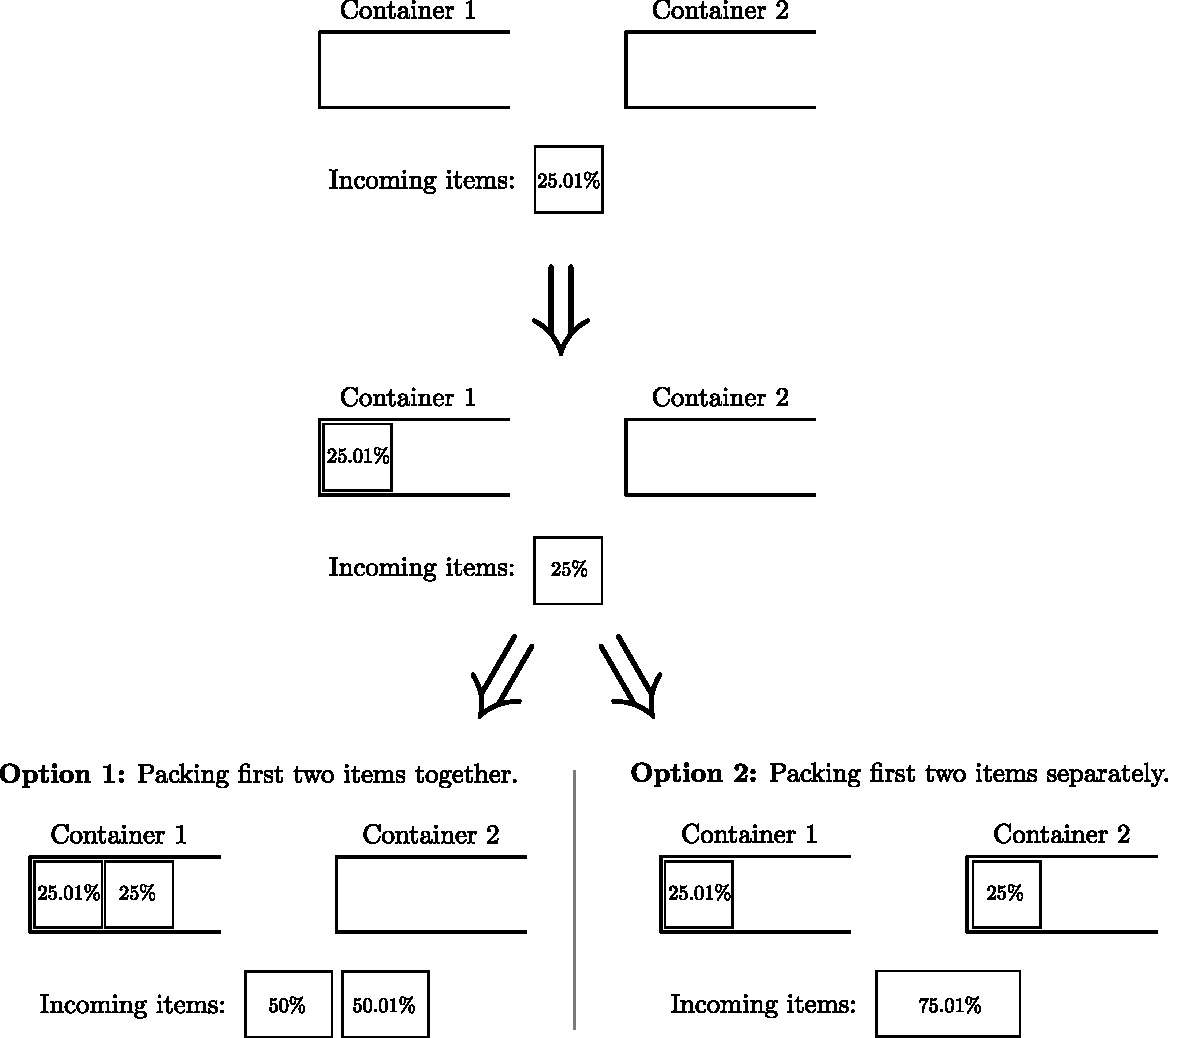
\includegraphics[width=\textwidth]{img/example-lowerbound.pdf}
\end{center}
\caption[A visual proof that two containers with original load of $75.01\%$ cannot
be repackaged without any reassignments.]{A visual proof that two containers with original load of $75.01\%$ cannot
be repackaged without any reassignments. A careful reader will observe that the number
of containers is not important here; a similar visual proof can be created for any
number of containers.}
\label{fig:example-lowerbound}
\end{figure}


% The most famous algorithmic problem dealing with online assignment is
% arguably {\sc Online Bin Packing}.  In this problem, known since the
% 1970s, items of size between $0$ and $1$ arrive in a
% sequence and the goal is to pack these items into the least number of
% unit-sized bins, packing each item as soon as it arrives.

% \binstretch, which has been introduced by Azar and Regev in
% 1998~\cite{azar98,azar01}, deals with a similar online
% scenario. Again, items of size between $0$ and $1$ arrive in a
% sequence, and the algorithm needs to pack each item as soon as it
% arrives, but there are the following differences: (i) The packing
% algorithm knows $m$, the number of bins that an optimal offline
% algorithm would use, and must also use only at most $m$ bins, and (ii)
% the packing algorithm can use bins of capacity $R$ for some $R\geq
% 1$. The goal is to minimize the stretching factor $R$.

% In general, the term ``semi-online'' refers to algorithms that,
% compared to online algorithms, have some additional global information
% about the instance of the problem or have another advantage. We have
% formulated \binstretch as a semi-online bin packing variant, where the
% algorithm has the additional information that the optimal number of
% bins is $m$ and at the same time the algorithm has the advantage of
% using bins of larger capacity.

% Taking another view, \binstretch can also be thought of as a
% semi-online scheduling problem, in which we schedule jobs arriving one
% by one in an online manner on exactly $m$ machines, with the objective
% to minimize the makespan, i.e., the length of the resulting
% schedule. Here the additional information is that the optimal offline
% algorithm could schedule all jobs with makespan $1$. Our task is to
% present an algorithm with makespan being at most $R$.

%\smallskip\noindent
%{\bf Motivation.} We give two applications of \binstretch.
%
%{\it Server upgrade.} This application has first appeared
%in~\cite{azar98}. In this setting, an older server (or a server
%cluster) is streaming a large number of files to the newer server
%without any guarantee on file order. The files cannot be split between
%drives. Both servers have $m$ disk
%drives, but the newer server has a larger capacity of each drive. The
%goal is to present an algorithm that stores all incoming files from
%the old server as they arrive.
%


% \todo{Below intro for threebins.}

% \section{Introduction}

% The most famous algorithmic problem dealing with online assignment is
% arguably {\sc Online Bin Packing}. In this problem, known since the
% 1970s, items of size between $0$ and $1$ arrive in a
% sequence and the goal is to pack these items into the least number of
% unit-sized bins, packing each item as soon as it arrives.

% \binstretch, which was introduced by Azar and Regev in 1998~\cite{azar98,azar01}, deals with a
% similar online scenario. Again, items of size between $0$ and $1$
% arrive in a sequence, and the algorithm needs to pack them as soon as
% each item arrives, but it has two advantages: (i) The packing
% algorithm knows $m$, the number of bins that an optimal offline
% algorithm would use, and must also use only at most $m$ bins, and (ii)
% the packing algorithm can use bins of capacity $R$ for some
% $R\geq 1$. The goal is to minimize the stretching factor $R$.

% While formulated as a bin packing variant, \binstretch can also be
% thought of as a semi-online sche\-du\-ling problem, in which we schedule
% jobs in an online manner on exactly $m$ machines, before any execution
% starts.  We have a guarantee that the optimum offline algorithm could
% schedule all jobs with makespan $1$. Our task is to present an online
% algorithm with makespan of the schedule being at most $R$.

% % \iffalse % motivation can be skipped to save space
% \subsection{Motivation} We give two applications of \binstretch.

% {\it Server upgrade.} This application has originally appeared
% in~\cite{azar98}. In this setting, an older server (or a server
% cluster) is streaming a large number of files to the newer server
% without any guarantee on file order. The files cannot be split between
% drives. Both servers have $m$ disk
% drives, but the newer server has a larger capacity of each drive. The
% goal is to present an algorithm that stores all incoming files from
% the old server as they arrive.

% {\it Shipment checking.} A number $m$ of containers arrive at a
% shipping center. It is noted that all containers are at most $p \le 100$ percent
% full. The items in the containers are too numerous to be individually
% labeled, yet all items must be unpacked and scanned for illicit and dangerous
% material. After the scanning, the items must be speedily
% repackaged into the containers for further shipping.
% In this scenario, an algorithm with stretching factor $100/p$
% can be used to repack the objects into containers in an online manner.
% % \fi

% \subsection{History}  
% \binstretch was first proposed by Azar and Regev in~\cite{azar98,azar01}.
% Already before this, a matching upper and lower bound of $4/3$ for two bins
% had appeared~\cite{KeKoST97}.
% %The original lower bound of $4/3$ for three bins has appeared even
% %before that, in~\cite{KeKoST97}, for two bins together with a matching
% %algorithm.  
% Azar and Regev extended this lower bound to any number
% of bins and gave an online algorithm with a stretching factor $1.625$.

% The problem has been revisited recently, with both lower bound
% improvements and new efficient algorithms. On the algorithmic side,
% Kellerer and Kotov~\cite{kellerer2013} have achieved a stretching
% factor $11/7 \approx 1.57$ and Gabay et al.~\cite{gabay2013} 
% have achieved $26/17 \approx
% 1.53$. The best known general algorithm with stretching factor $1.5$
% was presented by the authors of this paper in \cite{bsvsv16}.

% In the case with only three bins, the previously best
% algorithm was due to Azar and Regev~\cite{azar98}, with a stretching
% factor of $1.4$.

% On the lower bound side, the lower bound $4/3$ of~\cite{azar98} was
% surpassed only for the case of three bins by Gabay et
% al.~\cite{gabay2013lbv2}, who show a lower bound of $19/14\approx
% 1.357$, using an extensive computer search. The preprint
% \cite{gabay2013lbv2} was updated in 2015 \cite{gabay2013lbv3} to
% include a lower bound of $19/14$ for four bins.

% A preliminary version of this work appeared in WAOA 2014
% \cite{bsvsv14} and SOFSEM 2016~\cite{bohm16}.

% % \smallskip\noindent
% \subsection{Related work.} The NP-hard problem \binpacking was originally
% proposed by Ullman~\cite{ullman71} and Johnson~\cite{johnson73} in the
% 1970s. Since then it has seen major interest and progress, see the
% survey of Coffman et al.~\cite{coffman13} for many results on
% classical Bin Packing and its variants. While our problem can be seen
% as a variant of {\sc Bin Packing}, note that the algorithms cannot
% open more bins than the optimum and thus general results for
% \binpacking do not translate to our setting.

% As noted, \binstretch can be formulated as the online scheduling on $m$ identical
% machines with known optimal makespan. Such algorithms were studied and
% are important in designing constant-competitive algorithms without the
% additional knowledge, e.g., for scheduling in the more general model
% of uniformly related machines~\cite{AsAFPW97,BeChKa00,EbJaSg09}.

% For scheduling, also other types of semi-online algorithms are
% studied. Historically first is the study of ordered sequences with
% non-decreasing processing times~\cite{Graham69}. Most closely
% related is the variant with known sum of all processing times studied
% in~\cite{KeKoST97} and the currently best results are a lower bound of
% $1.585$ and an algorithm with ratio $1.6$, both
% from~\cite{DBLP:journals/tcs/AlbersH12}. Note that this shows,
% somewhat surprisingly, that knowing the actual optimum gives a
% significantly bigger advantage to the online algorithm over knowing
% just the sum of the processing times (which, divided by $m$, is a
% lower bound on the optimum).

